%% template for IEICE Transactions
%% v1.7new [2010/02/03]
\documentclass[paper]{ieice}
%\documentclass[invited]{ieice}
%\documentclass[survey]{ieice}
%\documentclass[invitedsurvey]{ieice}
%\documentclass[review]{ieice}
%\documentclass[tutorial]{ieice}
%\documentclass[letter]{ieice}
%\documentclass[brief]{ieice}
\usepackage[dvips]{graphicx}
\usepackage[fleqn]{amsmath}
\usepackage[varg]{txfonts}
\usepackage{url}
\usepackage{cite}
\usepackage{epsfig}
\usepackage{float}
\usepackage{caption}
%\usepackage{subcaption}
\usepackage{graphicx}
%\usepackage[ngerman]{babel}
%\usepackage[T1]{fontenc}
%\captionsetup[subfigure]{labelformat=parens, format=hang, margin=0pt, parskip=0pt,
%		hangindent=0pt, indention=0pt, singlelinecheck=false, textfont=footnotesize}

\setcounter{page}{1}
%\breakauthorline{}% breaks lines after the n-th author

\field{B}
%\SpecialIssue{}
\SpecialSection{on XXXYYYZZZ}
%\theme{}
\title{Towards Sustainable Content Delivery with Peer-Assisted CDN}
%
%\title[title for header]{title}
\authorlist{% fill arguments of \authorentry, otherwise error will be caused. 
 \authorentry[dikshie@sfc.wide.ad.jp]{{Mohamad Dikshie} Fauzie}{n}{labelA}
 \authorentry{{Achmad Husni} Thamrin}{n}{labelA}
% \authorentry{Rodney Van Meter}{n}{labelB}
 \authorentry{Jun Murai}{m}{labelB}
}
\affiliate[labelA]{The author is with Graduate School of Media and Governance Keio University, Fujisawa-shi, 252-0882 Japan }
\affiliate[labelB]{The author is with Faculty of Environment and Information Studies Keio University, Fujisawa-shi, 252-0882 Japan }

%\paffiliate[present affiliate label]{Presently, the author is with the }
\received{2010}{1}{1}
\revised{2010}{1}{1}
%\finalreceived{2010}{1}{1}

%% <local definitions here>
%% </local definitions here>

\begin{document}
\maketitle

\begin{summary}
Users watched video over Internet has increased and it should be anticipated by ISP.  
On the other hand ISP want to keep the cost of delivering contents to users is minimize.
\end{summary}
\begin{keywords}
P2P, CDN, Internet Service Providers, Content Providers, Game Theory 
\end{keywords}  

%%%%%%%%%%%%%%%%%%%%%%%%%% INTRODUCTION %%%%%%%%%%%%%%%%%%%%%%%%%%%%%%%%%%%
\section{Introduction}\label{intro}
In recent years due to the widespread of broadband Internet connections, user achieved the possibility of downloading and sharing their multimedia contents.
Furthermore, more advanced hardware with a reduction of computer costs allowed users to own a high performance PC to perform complex task.
More people are watching video on their PC using specific applications or plugins that integrated into browsers.
Common technical solution just rely on a client-server architecture.
This solution is not viable since it can not scale if the content becomes popular.
Some content companies have agreement with CDN (content delivery network) providers such as Akamai, Limelight, or Level3 to distributed the contents better scale and better QoE (quality of experience) to end users.
For example, Youtube uses Google cache, MTV uses Akamai, etc. P2P (peer to peer) applications are also widely deployed and their success is quite important. 
In China, P2P is very popular. 
We see many P2P applications from China such as PPLive, PPStream, UUSe, Xunlei, etc.  
Some news broadcaster are also rely on P2P technology to deliver popular live events.
For example, CNN uses Octoshape solution that enable to scale and offer good video quality while the number of users increase.
From Internet provider point of view, the diffusion of powerful computers in users side suggested that it could be possible to delegate a portion of computing or storage tasks to the users thus creating P2P networks where users can share files and multimedia contents.
Starting from file sharing only protocol, P2P architecture evolved toward video on demand and live events support. 

A P2P based architecture usually requires a sufficient number of nodes supplying the data (termed as seeders) to start the distribution process among the joining peers.
A peer usually offers low outbound streaming rate due to traditional asymmetrical DSL home connections) and hence multiple peers must jointly stream a media data to a requesting peer. 
The decentralized, uncoordinated operation implies that scaling to high number of peers comes with side effects.
Typical problem of a P2P streaming architecture are the low stream quality with undesirable disruptions, resources unfairness due to heterogeneous peer resources and high startup delay.
Moreover, current P2P applications are not aware of the underlying network and may conflict with the ISP routing policies and business model.

Nowadays, a number of P2P streaming applications have been designed, analyzed and deployed attracting a significant amount of users.
Research studies and deployment experiences have both demonstrated that P2P is a promising solution in terms of scalability and deployment costs.
On the other hand, the heterogeneous nature and unstable behavior of the peers contributing bandwidth and computational resources along with the networking issues are limit the commercial success of P2P video streaming applications.
Apart from P2P protocols, video contents can be efficiently distributed leveraging on services offered by managed networks architectures and CDN companies.
The major issue of CDN are high deployment cost and limited scalability in the long term.
Given the complementary features of P2P and CDN, in the last years some hybrid solutions have been proposed \cite{Huang:2008:UHC:1496046.1496064,4772628,Yin:2009:DDH:1631272.1631279} to take the best of both approaches.

In recent year, xDSL networks are deployed worldwide and broadband access network helps the P2P application to perform better.
In the coming years, FTTH will be massively deployed by network operators in order to offer to their customers and even larger access bandwidth.
As bandwidth increase, more the P2P systems is efficient since a peer can contribute much more. 

P2P architecture offers great potential for content providers to cost effectively distribute content by capitalizing network resources of end users.
It is economical superiority to the traditional client-server architecture and it has been demonstrated by lots of academic work and successful commercial systems \cite{Yin:2009:DDH:1631272.1631279}.
We believe more content providers will adopt P2P technology in the future. 

In the mentioned work, each end user device is involved directly in the P2P swarm.
In such cases, the installation of a software for the P2P engine in every end device is necessary and the user itself is directly involved in the content's swarm.
In such condition peers may result unstable and the swarm can be affected by rapid and frequent disconnections.
Furthermore, user's devices usually can contribute to the swarm with limited upload bandwidth and techniques developed in P2P to select neighboring peers are often unfriendly with ISP's routing policies.
Different topologies have been proposed in literature, where the collaborative mechanism for content distribution is created among more stable devices such as residential gateways which are still geographically close to the end users but directly owned and managed by ISPs. 
In such conditions, running on more stable and powerful device, each peer can contribute with more bandwidth to the content swarm with respect to traditional end-user P2P. 
Peer selection procedures can also managed directly by ISP, avoiding the traversal of multiple nodes across ISP boundaries.

In some recent works, the residential gateway (i.e a home gateway placed in home premise, serving several terminals within the home network but directly managed by ISP) is considered the central entity of such managed P2P infrastructure as describe in \cite{Misra:2010:IPS:1811099.1811064,Cha:2008:NTP:1855641.1855646}.
Since P2P traffic now decreasing and moving to cloud \cite{Labovitz:2010:IIT:2043164.1851194}, there is room from ISP to use user's home gateway as peer assisted CDN since users usually do more download rather than upload.
The user home gateway is always on 24 hours therefore this is perfect device to run peer assisted application.
ISP can give discount price to user's who wants their home gateway to be used as peer assisted by ISP and ISP can get benefit from peer assisted running in their customer home gateway to help their CDN.
With the growing interest to do inter-connect of CDN \cite{cdni,oceanproject} this architecture can give good benefit for ISP.    

In this paper, we study the incentive for ISP who adopt peer assisted CDN for streaming purpose and show the advantages to adopt peer assisted CDN. 

%\begin{figure}[tb]
%\begin{center}
%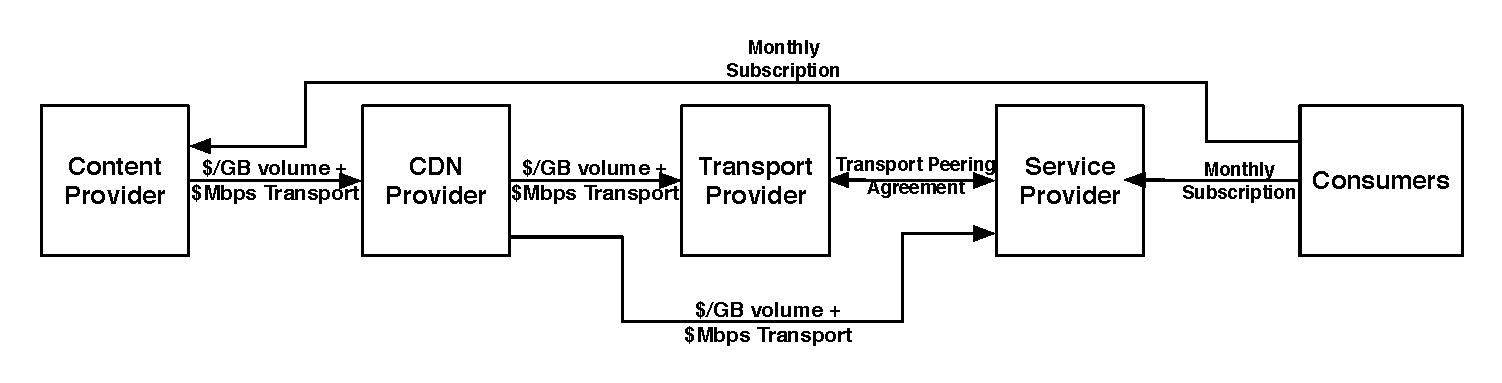
\includegraphics[scale=0.35]{graphs/today-ecosystems.eps}
%\end{center}
%\caption{Today Ecosystems.}
%\label{fig:todayeco}
%\vspace{-2mm}
%\end{figure}


%\begin{figure}[tb]
%\begin{center}
%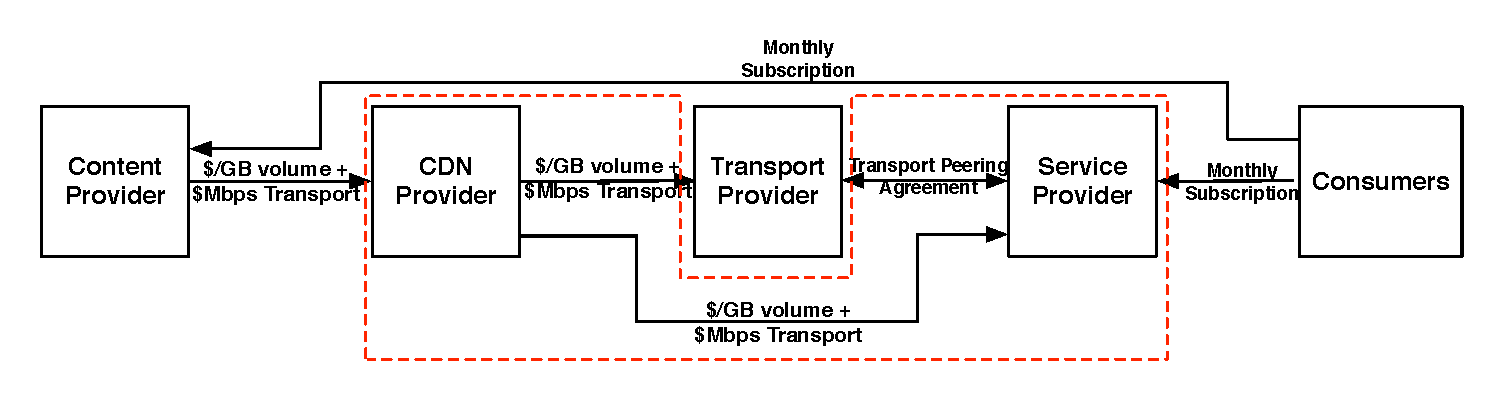
\includegraphics[scale=0.35]{graphs/today-ecosystems-sp.eps}
%\end{center}
%\caption{Today Ecosystems SP.}
%\label{fig:todayecosp}
%\vspace{-2mm}
%\end{figure}


\begin{figure}[tb]
\begin{center}
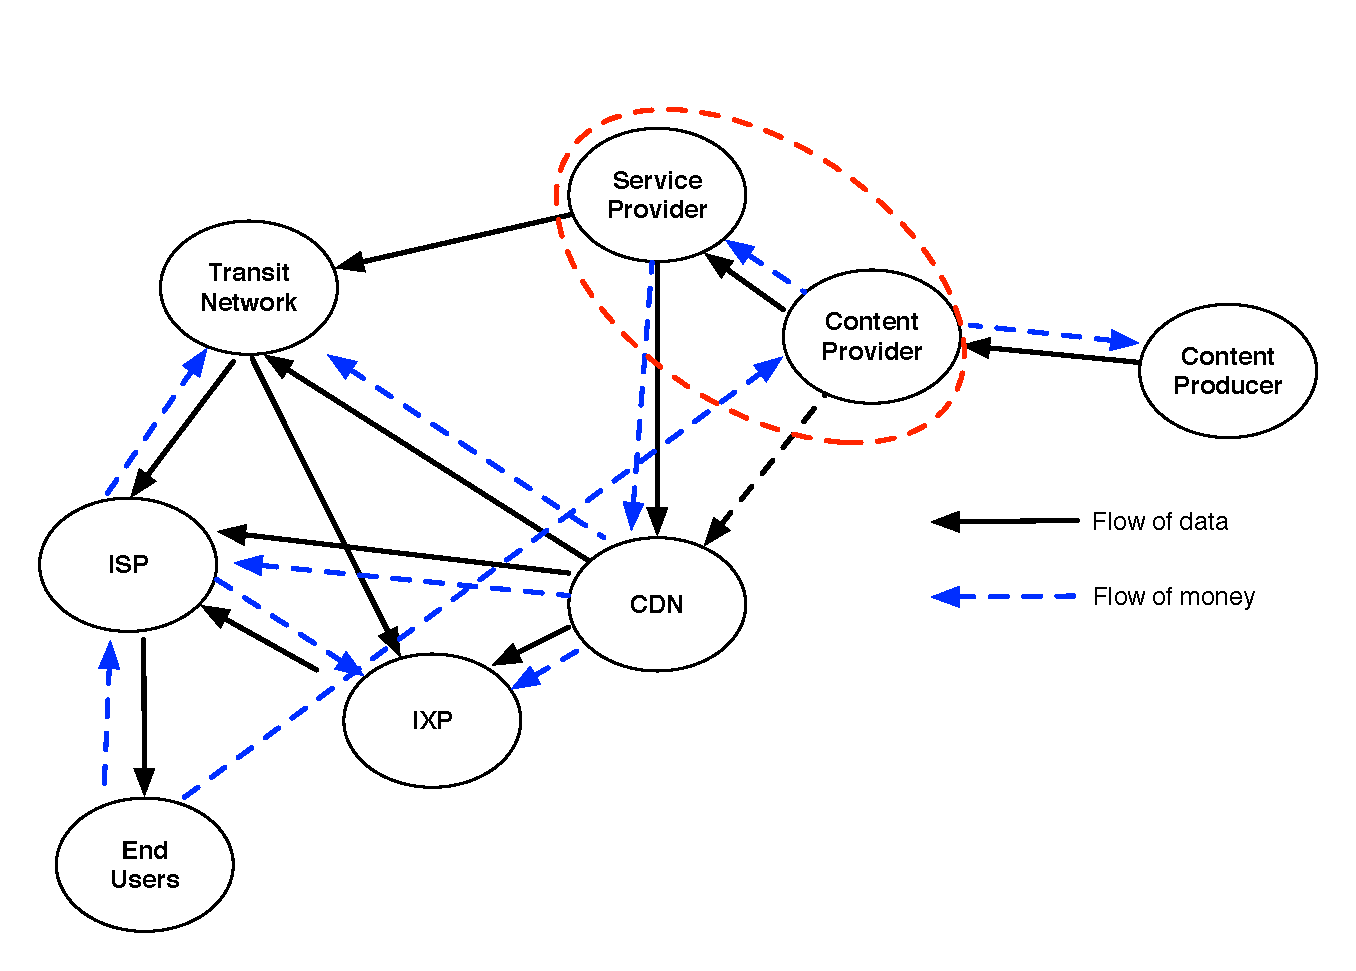
\includegraphics[scale=0.35]{graphs/business-relationship.eps}
\end{center}
\caption{Complex relationship of entities in Internet.The data flow from content producer to content provider. From content provider data can flow to service provider then goes to CDN. Depends on routing and peering policy, data from CDN can flow directly to ISP or flow to ISP via IXP (Internet Exchange) or via transit network. Flow of data noted by straight arrow and flow of money noted by dash arrow line.}
\label{fig:businessrelationship}
\vspace{-2mm}
\end{figure} 


%\begin{figure}[tb]
%\begin{center}
%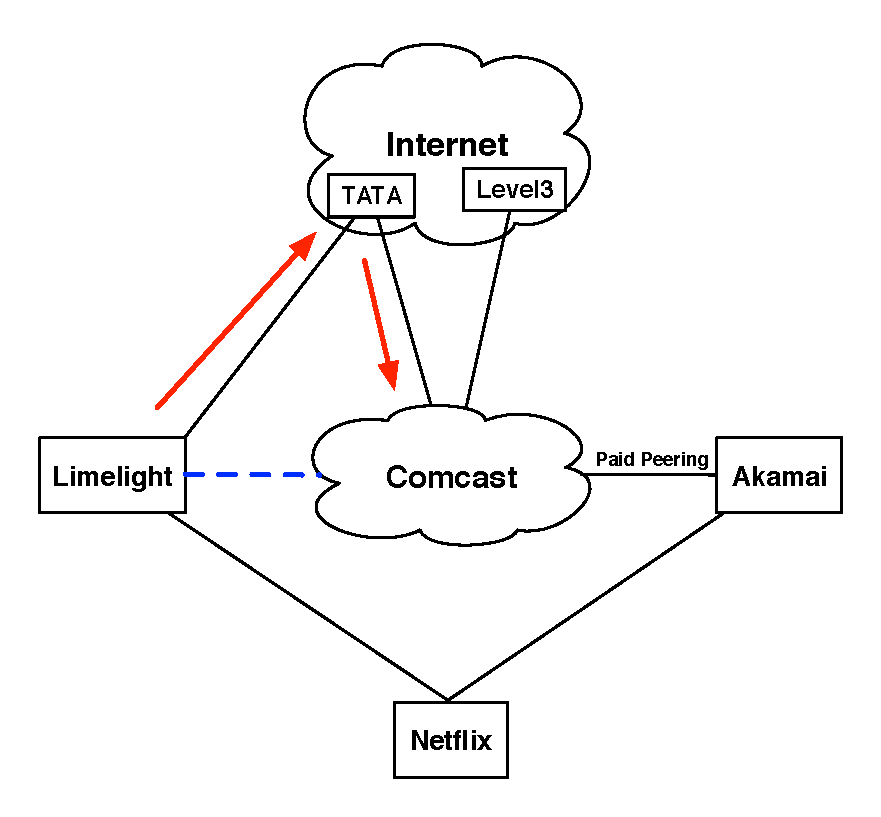
\includegraphics[scale=0.35]{graphs/llnw-tata-comcast.eps}
%\end{center}
%\caption{Akamai purchased paid peering from Comcast and enjoy low latency and high capacity access to Comcast's customers.
%Limelight use Tata to deliver contents to Comcast's customers (arrow line). 
%Due to high congestion on the link between Comcast and Tata, Netflix began to complain to Limelight because Netflix paid Limelight to deliver contents. 
%Finally Limelight purchased paid peering from Comcast (dash line).}
%\label{fig:llnw}
%\vspace{-2mm}
%\end{figure}

%\begin{figure}[tb]
%\begin{center}
%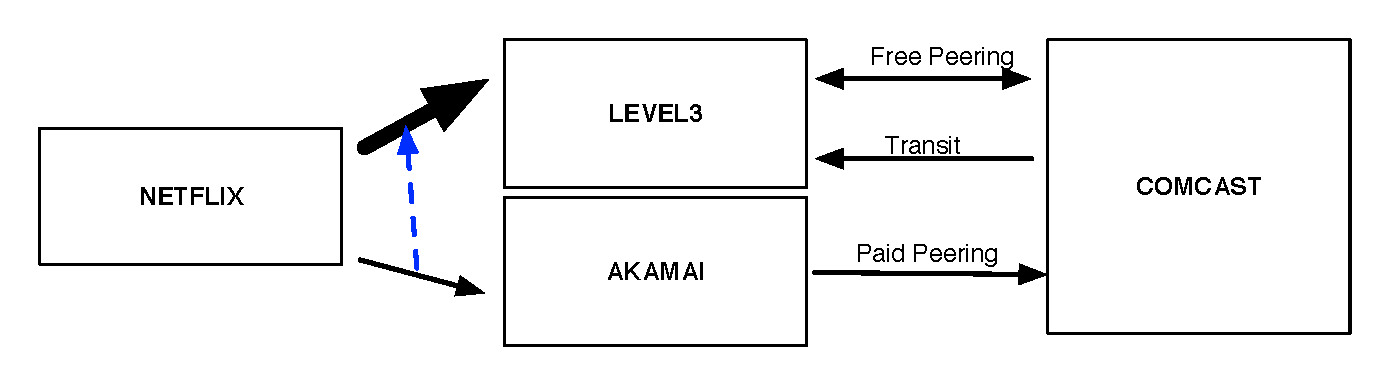
\includegraphics[scale=0.35]{graphs/comcast-level3.eps}
%\end{center}
%\caption{Level3 and Comcast has settlement free peering. Comcast is also use Level3 as transit network. 
%Netflix change its contents delivery network from Akamai to Level3 (arrow dash line).
%Level3 traffic to Comcast became out of ratio therefore Comcast asked Level3 to buy paid peering.}
%\label{fig:comcast}
%\vspace{-2mm}
%\end{figure}

%%%%%%%%%%%%%%%%%%%%%% CDN COMPLEXITY %%%%%%%%%%%%%%%%%%%%%%%%%%
\section{CDN Complexity}
As shown in Fig.\ref{fig:businessrelationship}, how content in Internet delivered to end-users.  
Content producer such as movies companies send their movies to content provider for example: Netflix and Hulu.
Content providers then deliver the movies using CDN or they also can use their upstream provider.
Depends on peering policies, CDN can reach to customer directly via ISP or via IXP then reach ISP or goes to transit networks then reach ISP.   
In current modern Internet topology, content provider and service provider can be merged in on entity, for example: Google.
Labovitz et al.,\cite{Labovitz:2010:IIT:2043164.1851194} mentioned that the hyper-giant entities such as Google doing massive peering to IXP in order to be closed to ISP. 
Although CDN is placed close to ISP network, it does not guarantee end-users can get good quality video stream \cite{Krishnan:2009:MBE:1644893.1644917}.
Other than technical complexity as mentioned before, CDN also faces economic complexity\cite{dispute}.
Therefore, the future of CDN business is likely to live deeper into ISP networks, more integrated into and interleaved with ISP infrastructures.

\begin{figure}[hb]
\begin{center}
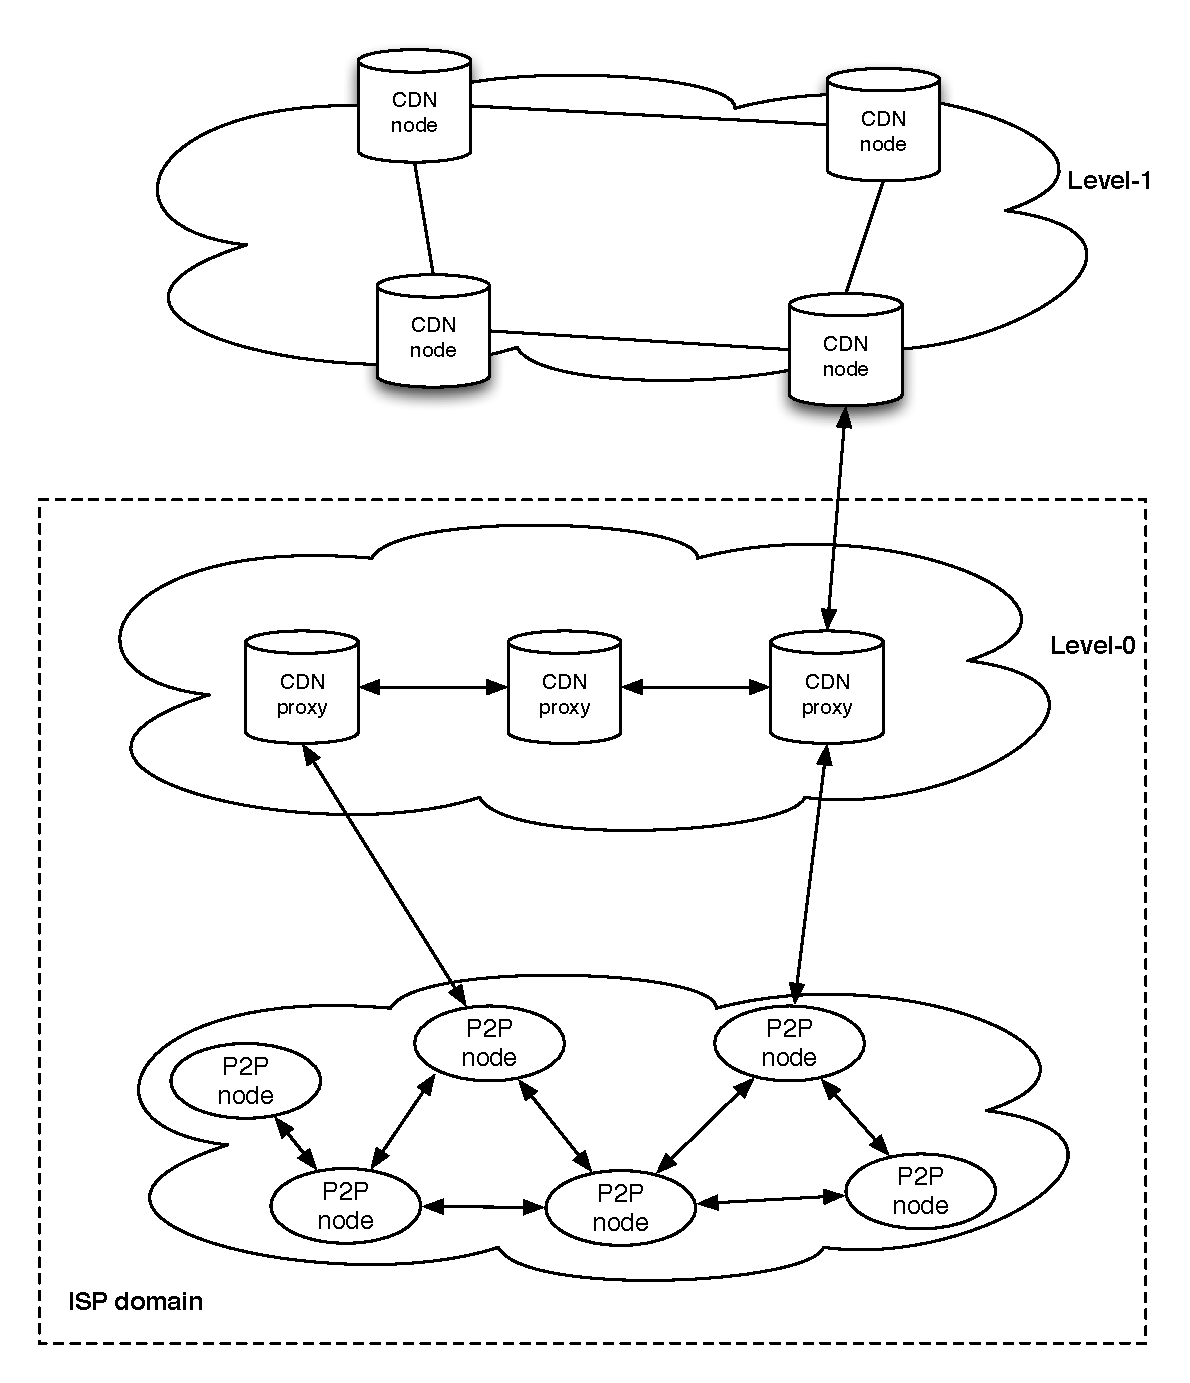
\includegraphics[scale=0.35]{graphs/two-tier-cdn-topology.eps}
\end{center}
\caption{Two tier CDN-P2P topology.
The CDN proxy maintained by ISP. ISP also has CDN node. CDN node can exchange contents with other CDN node owned by other CDN companies.P2P nodes are ISP's customers that run P2P software.}
\label{fig:twotier}
\vspace{-2mm}
\end{figure} 


 
%%%%%%%%%%%%%%%% %%%%%% SYSTEM DESCRIPTION %%%%%%%%%%%%%%%%%%%%%%%
\section{System Description}\label{description}

Figure \ref{fig:twotier} shows the model of system architecture.
That's model offers the opportunity to connect the P2P swarm not directly but through an intermediate later of proxies.
This function has potential benefit: boosting download performances (by exposing through proxy devices higher upload bandwidth than end users). 
It is also increasing privacy by reducing swarm exposure for end users.
This two level of CDN follows hierarchical model in Maki et al.,\cite{NaoyaMAKI2012} with modification.

The first level Level-1 consists high capacity servers strategically placed to increase network backbone capacity.
Level-1 is more like current CDN network.
In Level-1, CDN node can communicate each other by using common interconnect interface even though the CDN node are owned by different companies or different ISPs \cite{cdni}.

Level-0 consists CDN proxies are owned or to be managed by ISP.
For big ISP different CDN proxies in level-0 can be put at different cities or different geographically areas.
These nodes are placed closer to end users. 
CDN proxies can communicate each other to react to the content requests from users.
Level-0 are the natural service points for the users and they can offer the best quality of service if the are able to efficiently cache the requested content.
The state of the Level-0 and Level-1 caches is stored in DHT. 
The DHT is used to keep an updated record for each content in scalable manner. 
This different caching levels are used to offer an adaptive, flexible, and scalable service to the users.

We noted that CDN proxy has a limited capacity and it may not be able to satisfy all clients.
A peer-assisted CDN introduced peer coordination mechanism into CDN system. 
In this case CDN proxy is responsible to make peer coordination.  
For any new streaming request, the CDN proxy will have to make two decisions.
The CDN proxy will make a arrival node as seeder or as leecher based on adaptation strategy or a capacity constraint.  
In this system, we define a seeder is a node or a peer that receive stream from CDN proxy and a leecher is a node or a peer that receive stream from a seeder.  
To maintain low delay and good quality video streaming, seeder only receive stream directly from CDN proxy and leecher only receive from seeders.

It is very important for ISP to make sure CDN proxy capacity is enough while maintaining minimum capacity requirement. 
Although peer selection strategy is out of scope of this paper, we assume that peers form random mesh networks. 
In the next sections we will show how CDN proxy can make such decision in a way to optimize system.

%Other architecture, CDN federation proposed by Cisco and some ISPs to interconnect the ISP's CDN \cite{federation}.
%The goal CDN federation architecture is to interconnect ISPs owned CDN thus reduce Capex and Opex for content delivery. 
%This architecture does not involved P2P. 
%Some peering or transit might be needed by ISP to join this architecture. 
 

  
 
%%%%%%%%%% SYSTEM MODEL %%%%%%%%%%%%%%%%%%%%%%%%%%%
\section{System Model and Result Analysis}\label{systemmodel}
We present a model between P2P and CDN using simple a single bitrate for video streaming as shown in Fig.\ref{fig:twotier2}. 
The model is a stochastic fluid model similar to \cite{4215694}.
While the authors in \cite{4215694} focus on probability of degraded service on small and large systems, our work focus on minimum capacity or of CDN proxy to support the system.
Minimum capacity is very important to ISP for capacity planning.
On next subsection we also present a model of simple game theory between ISP who operate P2P-CDN and users.
We aim to find out the indifferent utility function between ISP and users.

\begin{figure}[tb] 
\begin{center}
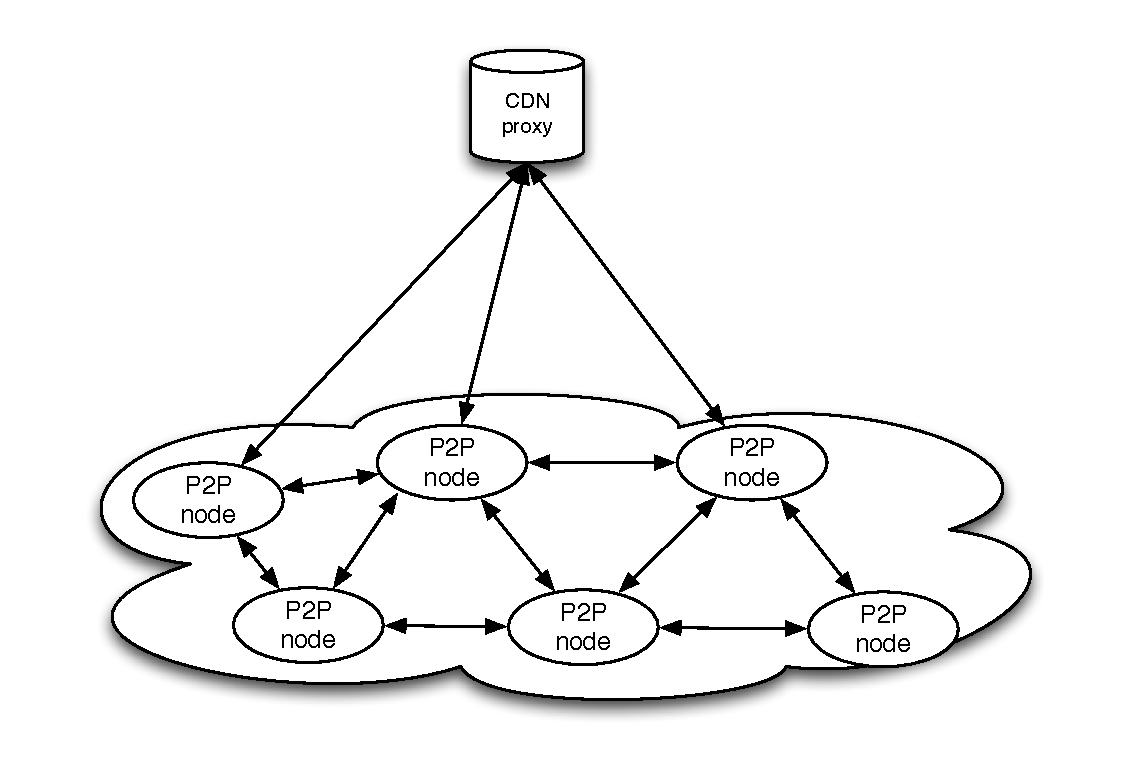
\includegraphics[scale=0.35]{graphs/two-tier-cdn-topology-2.eps}
\end{center}
\caption{System architecture on L0. P2P nodes that run on user home gateway communicates to CDN proxy.}
\label{fig:twotier2}
\vspace{-2mm}
\end{figure}

\subsection{Stable System}

For stable system, denote $n_l$ is the number of leechers, $n_s$ is the number of seeders in the system, and $r$ is bitrate.
Number of bitrate that leechers should receive is $n_l.r$. 
On the other hand seeders should upload to leechers which is $n_s.u_s$
We can derive that minimum CDN proxy capacity to support the system is:
\begin{equation}
	U_p = n_s.r + n_l.r - min(n_s.u_s, n_l.r)
\end{equation}
Based on leecher and seeder definition on Sec.\ref{description}, seeder already enjoyed direct streaming from CDN proxy with bitrate $r$ but upload rate of seeder to leecher might not same as streaming bitrate. 
That's the reason leecher may get source of video streaming from other seeders.  
Moreover, we define $X=\frac{n_l}{n_s}$ and normalization $r=1$ , we can get:
\begin{equation}
	\frac{U_p}{n_s} = (1 + X - min (u_s,X))
\end{equation}
Where $X$ is ratio number of leechers to number of seeders.
For CDN proxy can fulfill required capacity following inequality must be satisfied: $n_s.u_s \ge n_l.r$.
This inequality will be used in churn situation by CDN proxy to decide whether new arrival peers should be seeder or leecher.

\begin{figure}[hb] 
\begin{center}
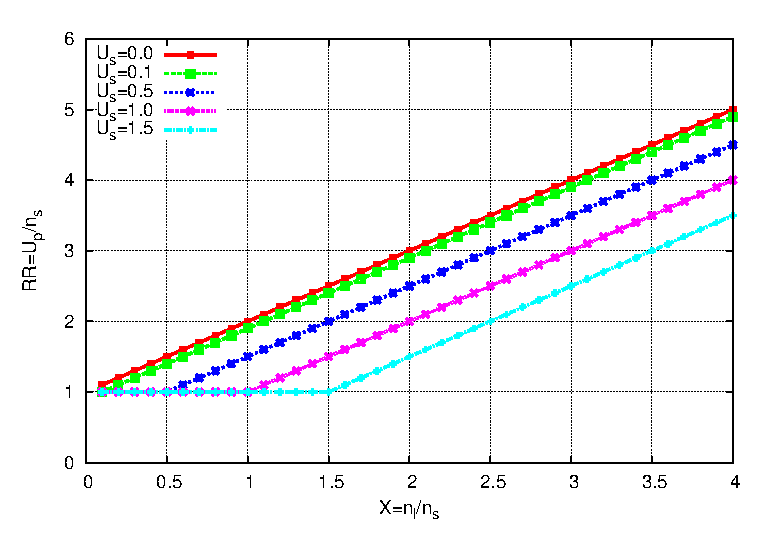
\includegraphics[scale=0.5]{graphs/stable-steady-state.eps}
\end{center}
\caption{System with steady state.}
\label{fig:steadystate}
\vspace{-2mm}
 \end{figure}
 
Figure \ref{fig:steadystate} shows steady state of the system without churn.
Lets take an example where $U_s=1.5$. The minimum of capacity CDN proxy to support the system can be achieved if the ratio between leechers to seeders less than 1.5.
Same with other $U_s$ value, as long as the ratio less than 'turning point' in the graph, that's the minimum of capacity that can be achieved to support the system.  
If the ratio more than 'turning point', the CDN proxy must add capacity to support the system thus add cost for ISP.

\begin{figure*}[thb]
\begin{minipage}[b]{0.4\linewidth}
\centering
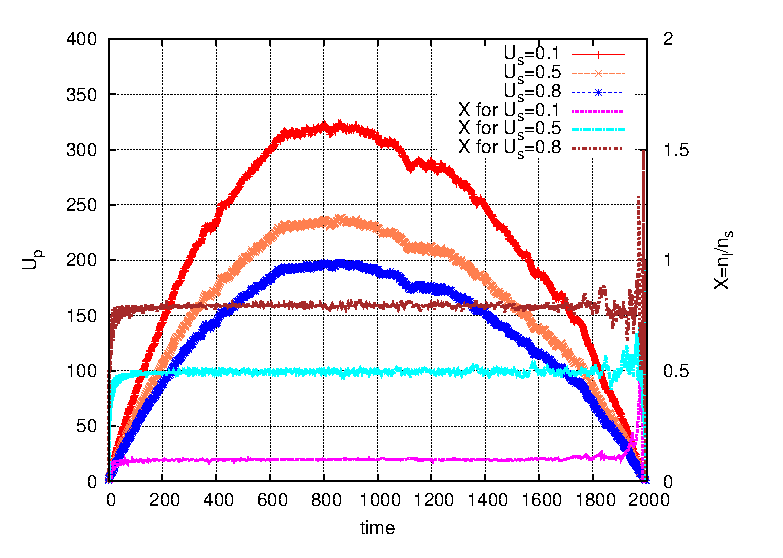
\includegraphics[width=2.7in]{graphs/U_p_n_1000.eps}
\caption{$U_p$ for $n=1000$ for admission policy 1.}
\label{fig:U_p_1000_1}
\end{minipage}
\hspace{0.5cm}
\begin{minipage}[b]{0.5\linewidth}
\centering
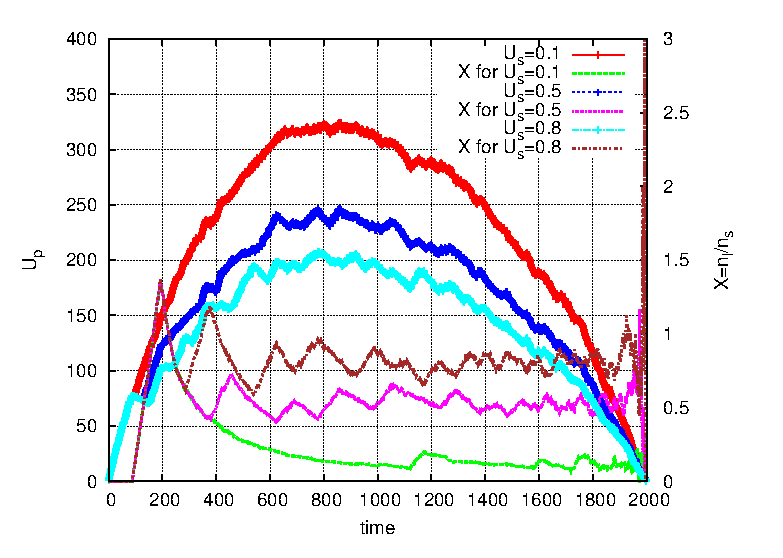
\includegraphics[width=2.7in]{graphs/U_p_n_1000_admi.eps}
\caption{$U_p$ for $n=1000$ for admission policy 2.}
\label{fig:U_p_1000_2}
\end{minipage}
\end{figure*}

\begin{figure}[hb] 
\begin{center}
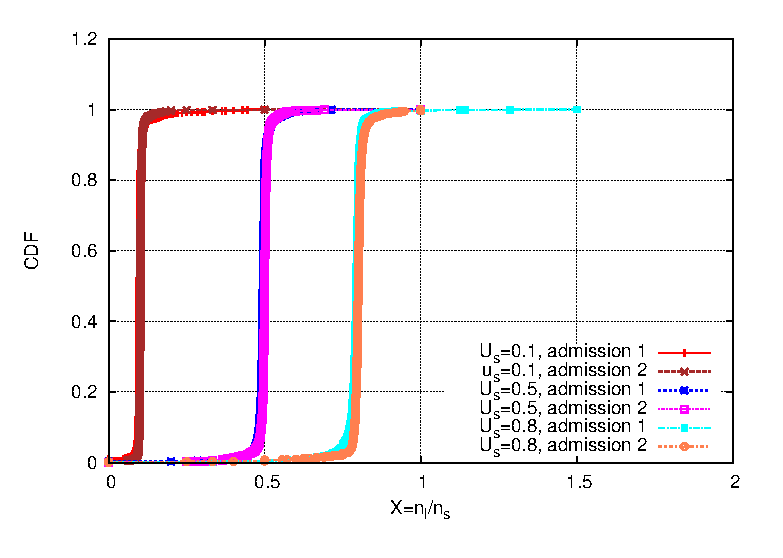
\includegraphics[scale=0.5]{graphs/cdf.eps}
\end{center}
\caption{CDF of $n_l/n_s$. We can see that admission policy 2 has bigger variance than admission policy 1.}
\label{fig:cdf}
\vspace{-2mm}
 \end{figure}
 
\subsection{Stable System with Churn}\label{sec:stablesystemwithchurn}
For churn case, we assume peers join and leave at random times, stay in for a random period, then leave the system.
Assuming poisson process with rate $\lambda$. 
Peers stay in the system for a period of time that follows a general probability distribution with mean $\frac{1}{\gamma}$.
Define $N(t)$ as the number of peers in the system at time $t$, $N(t)$ can be represented as the number of peers in a $M/G/\infty$ queue.
In poisson process, the time that these events occur in a given time interval. 
The time between each pair of consecutive events has an exponential distribution.
On the other hand, the number of events in time interval follows poisson distribution with rate $\rho = \frac{\lambda}{\gamma}$.
Now we can compute the probability of the probability of minimum capacity as following:
\begin{eqnarray*}
P(\text{support min capacity}) &=& P(\frac{U_p}{n_s} = 1+X-min(u_s,X))\\
&=&F(1+X-min(u_s,X))\\
\end{eqnarray*}
where $F=\sum_{x=0}^{w} \frac{e^{-\rho} \rho^{x}}{x!}$.
We know that for large $\rho$ we can approximate the poisson distribution with gaussian distribution with mean $\mu=\rho$ and standard deviation $\sigma = \sqrt{\rho}$, $F_{poisson}(x:\rho) \approx F_{normal}(x;\mu=\rho, \sigma^{2}=\rho)$.
We know that cumulative distribution function for standard normal random variable is $F(x) = \Phi(\frac{x-\mu}{\sigma})$ thus we can get:
\begin{eqnarray*}
P \left(\frac{(U_p/n_s) - \rho}{\sqrt{\rho}}=\frac{1+X-min(u_s,X) - \rho}{\sqrt{\rho}}\right)\\
=\Phi \left( \frac{1+X-min(u_s,X) - \rho}{\sqrt{\rho}} \right) \\
\end{eqnarray*}

In order CDN proxy handle the churn, we compare two different admission policy. 
First, the system starts admitting new arrivals as seeders until $(n_s.u_s > n_l.r)$. 
All arrivals after that point are admitted as leecher.     
Second, the system starts admitting new arrivals as seeders. 
Next the CDN proxy does polling mechanism on an interval time.
On that interval time CDN proxy decide the peers that arrives on that interval time to be seeder or leecher using $(n_s.u_s > n_l.r)$.

Figure \ref{fig:U_p_1000_1} shows $U_p$ values during simulation with total number of peers $N=1000$ and we use first admission policy in this simulation. 
We also plot ratio values $X$ on second Y-axis.
Fig.\ref{fig:U_p_1000_2} shows $U_p$ values during simulation with total number of peers $N=1000$ and we use second admission policy in this simulation.  
From both figures, we can see that first admission can stabilized the ratio $X$ in order to keep the CDN proxy capacity enough to supply the system since first admission try to decide peer role from beginning of peer arrival. 
In the second admission policy, CDN proxy decide peer role during time interval.
This make the ratio $X$ value of second admission policy has bigger variance.
To make it clear, Fig.\ref{fig:cdf} shows CDN of $X$ for $U_s=0.1, U_s=0.5, \text{and }  U_s=0.8$ for different admission policy. 
We can see that second admission gives bigger variance, while first admission can keep the ratio ideal.
Finally, we can see that seeder upload has big contribution for this system. 
This is become foundation for next section how to incentive peers in this system.




\subsection{ISP Strategies: Game Theory Approach}
In this section, we present simple game theory approach for analysis of ISP strategies.
Game theory as described in \cite{gametheory} is a mathematical framework to study and analysis of situation where decisions made by a set of two or more rational players.
Basic element of game are: rational players, strategies, and payoff or utility.  
Rational players choose a strategy for maximizing its payoff or utility. 
Extensive-form game is representation of corresponding decision nodes in a directed tree.
Later, we will use extensive-form game to represent our game.
In our model, ISP has already attempted to implement solution for peer-assisted CDN.
Moreover, it is reasonable to assume that ISP is naturally initiators.  
Stackelberg game also known as a leader-follower game is a class of game that concerns with situation where one player, the leader, initiates the decision making and where the second player, the follower, responds to the actions by the leader.  
Moreover in our model, ISP can be modeled as leader who decided to implement peer-assisted or not according to their expected payoff, while users can be modeled as followers that evaluate the decision of the ISP and responds according to their available actions and payoffs.

\newtheorem{theorem}{Definition}
\begin{theorem}[ISP Strategies]
We define the pure strategy space $S_{isp}$ to include two strategies combination choice $s \in \{CDN, CDN-P2P\}$ and corresponding subscription free $P^{s}$.
Futhermore, we denote the strategies as:
\begin{itemize}
	\item $s_1 = (CDN, P^{s_1})$ : the ISP decides to use CDN only and thus keeps charging the initial subscription free $P^{s_1}$.
	\item $s_2 = (CDN-P2P, P^{s_2})$ : the ISP decides recommends peer-assisted and offers a subscription fee $P^{s_2} \le P^{s_1}$.
\end{itemize}
Where the ISP strategy space $S_{isp} = \{s_1,s_2\}$.
\end{theorem}

After defined the strategy space of ISP, now we will describe user reaction.
User reactions can be accept ISP strategy or decline ISP strategy.  
If ISP decides to use CDN only then user can only accept ISP strategy.  
If ISP decides to employ peer-assisted CDN then user can accept ISP strategy or decline ISP strategy.

\newtheorem{theorem2}{Definition}
\begin{theorem}[User Strategies]
Given a ISP strategy decision $s$, possible user actions:
\begin{itemize}
\item $\hat{s_a}$: User accepts ISP strategy $s \in S_{isp}$.
\item $\hat{s_d}$: User decline ISP strategy $s$ when $s\in{s_2}$.
\end{itemize}
\end{theorem}
We describe that situation as extensive form in Fig.\ref{fig:gametree}.

\begin{figure}[tb] 
\begin{center}
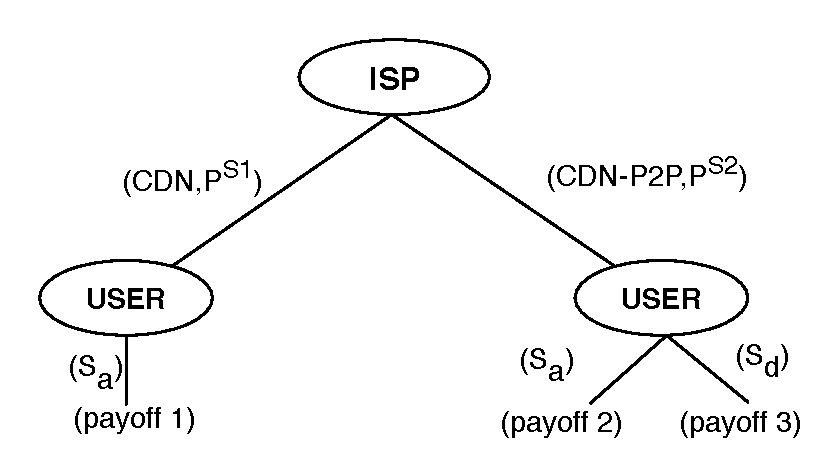
\includegraphics[scale=0.35]{graphs/game-tree.eps}
\end{center}
\caption{Extensive form of game between ISP and users}
\label{fig:gametree}
\vspace{-2mm}
\end{figure}

\subsubsection{ISP Payoff}
Next, we describe payoff function for ISP in our model.  
We assume a profit maximizing ISP that gains higher utility proportionally with increasing profits. 
A simplified business model that determining ISP payoff are mainly: user generated revenue and bandwidth cost to reach the users.

For revenue model, we assume that the ISP collects revenue solely by charging an initial flat rate subscription fee $P^{(s_1)}$ to its $N$ homogeneous users who are purchasing internet access with equal and fixed quality of service.
ISPs are often price discriminatory towards its customers and thus operates with different price levels for different speed or QoS.
ISPs are also get revenue from other business area such as email hosting, web hosting, etc. 
In our model, we do not include such that revenue. 
In order to keep simple, we found it reasonable only to focus on users that buy the same internet access product. 
Given above simplifications, the ISP collects a total revenue (when deciding on a strategy $s$) of $R = N P^{(s)}$.

For cost model, we identified that bandwidth cost to reach users is the most relevant aspect. 

\newtheorem{theorem3}{Definition}
\begin{theorem}[Bandwidth cost]
we define the bandwidth cost $\tau^{(s)}$ for a given ISP strategy $s$ to be denoted as 
\begin{equation}\label{eq:transitcost}
	\tau^{(s)}_t = \alpha^{(s)}T^{(s_1)} p_t
\end{equation}
where:
\begin{itemize}
	\item $T^{(s_1)}$ represent the average ISP traffic volume in Mbps to users.
	\item $\alpha^{(s)}$ represent the expected reduction factor for strategy $s$ such that: $\alpha^{(s)} \in [0,1]$ for $s \in \{s_2\}$;  $\alpha^{(s_1)} = 1$.
	\item $p_t$ represent the price of traffic.
\end{itemize}
\end{theorem}

In addition to the traffic costs, we also assume that ISP needs investment cost for peer-assisted CDN.
More specifically refer to Fig.\ref{fig:twotier2} ISP required to setup their Level-0 or CDN proxy and also provide different home gateway for users.

\newtheorem{theorem4}{Definition}
\begin{theorem}[Investment cost]
We define the investment cost $C^{(s)}_i$ to be a monthly amortization of a larger implementation related cost for the case when the ISP decides to implement peer-assisted. 
We denote:
\begin{align}
	C^{(s)}_i &\ge 0; \text{ for } s = s_2 \\
	          &= 0; \text{ for } s \in \{s_1\}
\end{align}
\end{theorem}

Finally after we defined all ISP cost, we can define ISP payoff function that will be used to model ISP utility.  

\newtheorem{theorem5}{Definition}
\begin{theorem}[ISP payoff]
We define the ISP payoff function $\pi_{isp}$ as:
\begin{align}\label{eq:isppayoff}
	\pi_{isp}^{(s)} &= N P^{(s)} - \tau^{(s)} - C_i^{(s)} \\
\end{align}
\end{theorem}

\subsubsection{User Payoff}
In this subsection, we  analyzed how the utility of user that purchases internet access at a fixed subscription fee $P^{(s)}$ can be described and derived. 
We assume that all users pay a fixed flat rate subscription fee $P$ for internet access with equal speed or QoS parameters.
Since users are rational player and subject to budget constraint, there must be a set of feature of internet access that valuable to users.
We assume one important parameter that describes the quality of an internet access product as perceived by customer is the perceived performance of internet applications.  
Moreover, the implementation of peer assisted mainly to reveal improvements of download speed as the performance metric that can be observed by customers.
Consequently, we make assumption that the user perceived quality of internet access increases proportionally with increases in peer assisted implementation. 

\newtheorem{theorem6}{Definition}
\begin{theorem}[User perceived quality]
we define the user perceived quality $Q^{(s)}$ of the internet access given an ISP strategy $s$ to be a function of speed that user received from ISP.
Moreover it is assume that the user initially perceived quality $Q^{(s_1)}$ is known. 
We formally denote $Q^{(s)}$ as:
\begin{equation}\label{eq:basicuserutility}
	Q^{(s)} = Q^{(s_1)}
\end{equation}
\end{theorem}

Therefore, given the assumption of proportional utility contribution from quality and price, we can define basic utility $U^{(s)}$. 

\newtheorem{theorem7}{Definition}
\begin{theorem}[Basic user utility]
We define basic utility $U^{(s)}$ a customer receives from buying internet access, given an ISP strategy decision $s$ as:
\begin{equation}
	U^{(s)} = Q^{(s)} - P^{(s)}
\end{equation}
Where $Q^{(s)} > P^{(s)}$.
\end{theorem}

User tends to accept reduction or discount.   
In order to keep P2P node on and keep the reward run to loyal users, ISP introduce penalty cost to users.
User get penalty cost from ISP if user turns off his/her home gateway.
We can define penalty cost as: 
\newtheorem{theorem8}{Definition}
\begin{theorem}[Penalty]
We define penalty as number of hours user home gateway per month multiply basic subscription fee.
\begin{equation}
	C_p = \frac{\text{number per hours off}}{30*24}.P^{(s)}
\end{equation}
Where $s\in\{s_2\}$
\end{theorem}

Finally, General form user payoff function (user accepts ISP strategy $s$):
\begin{equation}
	\pi^{(\hat{s_a} | s)}_u = U^{(s)} - C_p
\end{equation}
Where $C_p$ is penalty cost if user accept ISP strategy $s_2$ and $C_p=0$ if user accept ISP strategy $s_1$ or user decline ISP strategy $s_2$.

General form user payoff function:
\begin{itemize}
	\item User accepts ISP strategy $s_1$: 
	\begin{equation}
		\pi^{(\hat{s_a} | s_1)}_u  = U^{(s)}
	\end{equation}
	\item User accepts ISP strategy $s_2$: 
	\begin{equation}
		\pi^{(\hat{s_a} | s_2)}_u  = U^{(s)} - C_p
	\end{equation}
\end{itemize}

%by substitution basic user utility in Eq.\ref{eq:basicuserutility}, we can get general user payoff function:
%\begin{equation}
%	\pi^{(\hat{s_a} | s)}_u  = Q^{(s_1)} - P^{(s)}	
%\end{equation}

\subsubsection{Analytical Equilibrium Analysis}
As defined in previous section, both users and ISP are modeled as selfish players that maximize their utility (payoff) defined in the payoff functions.
As a consequence, an incentivizing strategy for both users and ISPs is a strategy that yields higher payoff then the other available strategies.
The ISP acting as a leader and initiator of the decision making, decides, on strategy $s$ that includes both a choice of technology as well as price offer $P^{(s)}$ which affect both ISP and user payoff.

From the user payoff function, we can observe that a user receives higher payoff as price decreases and will prefer lower prices.
The ISP on the other hand will naturally have a minimum limit for the subscription price as it, in our model, represents the only source of revenue.

Moreover we say that the minimum price $P^{(s)}_{min}$ that makes an ISP indifferent between strategy $s \in \{s_2\}$ and strategy $s_1$ can be found by identifying where the payoff of strategy $s$ equal the payoff of strategy $s_1$. 
That is expressed formally as:

\begin{equation}\label{ispminprice}
	\pi^{(s)}_{isp} = \pi^{(s_1)}_{isp}
\end{equation}
Where $s \in \{s_2\}$. 
Later Eq.\ref{ispminprice} can be written as: 

\begin{equation}\label{eq:ispminprice2}
	N P^{(s)}_{min} - \tau^{(s)} - C^{(s)}_i = N P^{(s_1)} - \tau^{(s_1)}  
\end{equation}
When subtituting payoffs with Eq.\ref{eq:isppayoff}, by furthermore solving Eq.\ref{eq:ispminprice2} for $P^{(s)}_{min}$ we can get:
\begin{equation}\label{eq:ispminprice3}
	P^{(s)}_{min} = P^{(s_1)} - \frac{1}{N} ( \tau^{(s)} - \tau^{(s_1)} +  C^{(s)}_i  )
\end{equation}

Given the above equations, we have found an expression for $P^{(s)}$ that express the point at which the ISP is indifferent to strategy $s$ over $s_1$ and thus represent the lower boundary for where both the users that ISP might have incentives for strategy $s$. 
Above equation can also express that ISP at maximum are willing to reduce its initial price $P^{(s_1)}$ by the expression $\frac{1}{N} ( \tau^{(s1)} - \tau^{(s)} -  C^{(s)}_i  )$.

It can be interpreted as a combination of the reduction in ISP total costs and investment.
Naturally, the implementation of peer assisted is assumed to reduce traffic cost.  
Futhermore, we can make observation that $\frac{1}{N} ( \tau^{(s1)} - \tau^{(s)} -  C^{(s)}_i )$ represents the maximum price reduction that an ISP might give. 
We can express how greedy an ISP is by introducing an parameter $\gamma$ that tells us what percentage of the maximum price reduction above an ISP is willing to share.  

\newtheorem{theorem9}{Definition}
\begin{theorem}[ISP price reduction]
Given observations above we can define the ISP price reduction $\theta^{(s)}$ when choosing strategy $s$ to be:
\begin{equation}
 \theta^{(s)} = \frac{\gamma}{N} ( \tau^{(s1)} - \tau^{(s)} +  C^{(s)}_i  )
\end{equation}
Where $\gamma \in [0,1]$ is a ratio that express how much of the ISP expected utility increase it wants to share with its users.   
We can also say that $\gamma$ represents the greediness of the ISP.
\end{theorem}

We now turn to the users perspective.  
Although, we assume that the ISP will offer a reduced subscription free when deciding to use peer-assisted, we will examine the more general maximum limit for $P^{(s)}$ from the user perspective.
We examine the case strategy $s \neq s_1$.
The maximum limit of $P^{(s)}$ can be expressed by:
\begin{equation}\label{eq:usermaxprice}
	\tau^{(s_a|s)}_u = \tau^{(s_a|s_1)}_u
\end{equation}
Where $s \in \{s_2\}$. Later Eq.\ref{eq:usermaxprice} can be written as:
\begin{equation}
	Q^{(s_1)} ( 1 + d^{(s)} ) - P^{(s)}_{max} = Q^{(s_1)} - P^{(s_1)}
\end{equation}
Futhermore we can get $P^{(s)}_{max}$:  
\begin{equation}\label{eq:usermaxprice2}
	P^{(s)}_{max} = P^{(s_1)} + Q^{(s_1)} d^{(s)}
\end{equation}
We found that the maximum value of the subscription free $P^{(s)}$ depends on the perceived performance increase $Q^{(s_1)} d^{(s)}$.

\newtheorem{theorem11}{Definition}
\begin{theorem}[Minimum-maximum subscription fee interval]
Next, we define minimum-maximum interval of the subscription fee $P^{(s)}$ as a value space of the subscription free where both ISP and users are expected to have incentives to adopt strategy $s$ as follows:
\begin{equation}
	P^{(s)}_{min} < P^{(s)} < P^{(s)}_{max}
\end{equation}
later by subtitution Eq.\ref{eq:ispminprice3} and \ref{eq:usermaxprice2} we can get:
\begin{equation}\label{eq:min-max-interval}
	P^{(s_1)} - \frac{1}{N} ( \tau^{(s1)} - \tau^{(s)} -  C^{(s)}_i  ) < P^{(s)} <  P^{(s_1)} + Q^{(s_1)} d^{(s)} 
\end{equation}
\end{theorem}


We analyze ISP level strategy among its strategies.
The ISP is indifferent between peer-assisted $(s_2)$ and CDN $(s_1)$ when $\pi^{(s_2)}_{isp} = \pi^{(s_1)}_{isp}$
which by using ISP payoff function in Eq.\ref{eq:isppayoff} can be written as: 
\begin{equation}
	N P^{(s_2)} - \tau^{(s_2)} = N P^{(s_1)} - \tau^{(s_1)}
\end{equation}
When we assume that the ISP will provide a lower subscription free when recommending peer-assisted such that $P^{(s_2)} < P^{(s_1)}$, we can use our findings on the ISP price reduction to present $P^{(s_2)}$ as:
\begin{eqnarray}
	\nonumber P^{(s_2)} &=& P^{(s_1)} - \theta^{(s_2)} \\
	P^{(s_2)} &=& P^{(s_1)} - \frac{\gamma}{N} (\tau^{(s_1)} - \tau^{(s_2)} - C^{(s_2)}_i )
\end{eqnarray}
The strategy restrictions as follows:
\begin{itemize}
	\item Choose strategy $s=s_2$ if $ P^{(s_2)} + \frac{\gamma}{N} (\tau^{(s_1)} - \tau^{(s_2)} - C^{(s_2)}_i ) > P^{(s_1)}$
	\item Choose strategy $s=s_1$ if $ P^{(s_1)} > P^{(s_2)} + \frac{\gamma}{N} (\tau^{(s_1)} - \tau^{(s_2)} - C^{(s_2)}_i )$ 
\end{itemize}

\subsubsection{Numerical Result}
In this subsection we do numerical evaluation the game theoretic model. 
The difficulty of doing numerical simulation is to assign right parameter values.
Simplyfing limitations that we use: 
\begin{itemize}
	\item We assume an ISP with $N=1000,10000,100000$ homogeneous users that pay an equal subscription fee $P^{(s_1)}$.
	\item We assume that inter ISP traffic is generated by video traffic and the traffic is distribution between one transit provider and one paid peering provider.
	\item We assume that user utilize $100\%$ of their internet connection capacity.  
\end{itemize}


%%%%%%%%%%%%%%%%% RELATED WORK %%%%%%%%%%%%%%%%%%%%%%%%
\section{Related Work} 
Content distribution network with peer-assisted have been successfully deployed on the Internet an example Akamai \cite{Huang:2008:UHC:1496046.1496064} and LiveSky \cite{Yin:2010:LEC:1823746.1823750}.
The Authors of \cite{Huang:2008:UHC:1496046.1496064} from two real world traces conclude that hybrid CDN-P2P can significantly reduce the cost of content distribution and can scale to cope with exponential growth of Internet video content.
Yin et al., \cite{Yin:2010:LEC:1823746.1823750} described commercial operation of CDN with peer-assisted in China.   
LiveSky solved several challanges in the system design such as dynamic resources scaling of P2P, low startup latency of P2P, ease of P2P integration with existing CDN infrastructure, and network friendliness and upload fairness in the P2P operation. 
Xu et al.,\cite{DBLP:journals/corr/abs-1212-4915} using game theory shows that right cooperative profit distribution of P2P can help ISP to maximize the utility. 
Their model can easily implemented to current Internet economic settlement.
Misra et al.,\cite{Misra:2010:IPS:1811099.1811064} also mentioned the important of P2P architecture to support content delivery networks. 
The author uses cooperative game theory to formulate simple compensation rules for users who run P2P to support content delivery networks.  

The idea telco or ISP managed CDN has been soared in recent years.  
The complexity of CDN business leads telco and ISP want to managed their own ISP.
It has been shown that it is cost effective \cite{federation}\cite{norton2011internet}. 
Kamiyama et al., \cite{NoriakiKAMIYAMA2013} proposed optimally ISP operated CDN. 
Kamiyama et al., mentioned that to deliver large and rich Internet content to users, ISP needs to put their CDN in data center.
The locations are limited while the storage is large, makes this solution become effective, using optimum placement algorithm based on real ISP network topologies.
The authors found that inserting CDN to ISP's ladder-type networks is effective to reduce the hops length thus reduce total link cost. 
On the other hand, an effort for telco or ISP managed CDN to be connected each other has been also initiated by Cisco to form CDN federation \cite{federation} using open standard \cite{cdni}.
They argue that current CDN architecture is not enough closer to the users and ISP can fill this position.   

The idea to utilize users computation power to support ISP operation is not new.  
European via Figaro project \cite{figaro} proposed residential gateway as integrator of different networks and services and become Internet-wide distributed content management for future Internet architecture \cite{figaro}. 
Cha, et al.,\cite{Cha:2008:NTP:1855641.1855646} did trace analysis and found that IPTV architecture powered by P2P can handle much larger number of channels with limited demand for infrastructure compare to IP multicast. 
Jiang et al., \cite{Jiang:2012:OMD:2413176.2413193} proposed scalable and adaptive for content replication and request routing for CDN servers that located in users home gateway. 
Our work close to Maki et al.,\cite{NaoyaMAKI2012} work.  
Maki et al.,\cite{NaoyaMAKI2012} propose traffic engineering for peer-assisted CDN to control the behavior of clients and presents a solution for optimizing the selection of content files.
Our work is a little bit same in system model architecture which uses different level of topologies which L0 and L1 where is Maki et al., \cite{NaoyaMAKI2012} the authors uses different name which is local domain and global domain. 
While our work focus on fluid limit for number of peers needed to support intended bit rate in single bit rate system and modeling simple economic incentive for ISP, Maki et al., \cite{NaoyaMAKI2012} work focus on algorithm of traffic engineering for optimizing selection of content files and controlling behavior of clients.

%%%%%%%%%%%%%%%%% CONCLUSION %%%%%%%%%%%%%%%%%%%%%%%%%
\section{Conclusion and Future Work}\label{conclude}
This paper presents scheme for peer-assisted ISP managed CDN model that estimate lower bound of peers based on stochastic fluid model and estimate the economic incentive for ISP based on game theory.  
Our numerical result shows that peer-assisted CDN managed by ISP or telco is feasible to deploy and does not harm to ISP business. 
Our future work will include energy efficient trade off this peer-assisted ISP managed CDN. 
We are very interested to know how much energy saving by ISP and how much increase of energy at users home gateway side in this architecture. 





%%%%%%%%%%%%%%%%% ACKNOWLEDGEMENT %%%%%%%%%%%%%%%%%%%%%
\section*{Acknowledgements}
We thank Joe Touch for suggestions.


\bibliographystyle{ieicetr}% bib style
\bibliography{jurnal}% your bib database

%\begin{thebibliography}{99}% more than 9 --> 99 / less than 10 --> 9
%\bibitem{}
%\end{thebibliography}

\profile[]{Mohamad Dikshie Fauzie}{%
was born in 1976. 
He received a bachelors degree and a master's degree from Institute of Technology Bandung, Indonesia.
He is currently a Ph.D candidate at Keio University's Shonan Fujisawa Campus.
}

\profile[]{Achmad Husni Thamrin}{%
is Assistant Professor at Keio University. 
He is a graduate of Keio University, Graduate School of Media and Governance (Ph.D 2005, MMG, 2002). 
His research interests include multicast, Internet over broadcast media, and peer-to-peer networks.
}

%\profile[photos/a3.eps]{Rodney Van Meter}{%
%received a B.S. from the California Institute of Technology in 1986,
%an M.S. from the University if Southern California in 1991, and
%a Ph.D. from Keio University in 2006. His research interests include
%storage systems, networking, post Moore's law computer architecture,
%and quantum computing. He is an Associate Professor of Environment and
%Information Studies at Keio University's Shonan Fujisawa Campus.
%}
\profile[]{Jun Murai}{%
was born in March 1955 in Tokyo. Graduated Keio University in 1979,
Department of Mathematics, Faculty of Science and Technology.
He received his M.S. for Computer Science from Keio University in 1981,
and received his Ph.D. in Computer Science, Keio University in 1987. 
He specializes in computer science, computer network, and computer 
communication. He is currently Dean of the Faculty of Environment and
Information Studies, Keio University since October 2009. Former
Vice-President of Keio University from May 2005 to May 2009. He was
an Executive Director of the Keio Research Institute at SFC, Keio
University from 1999 to 2005.
}
 
\end{document}
